\begin{marginfigure}[7cm] %MARGIN FIGURE
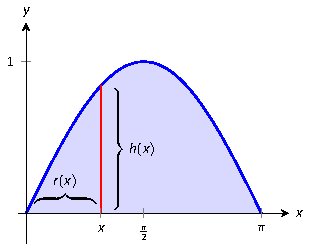
\includegraphics{figures/figshell4a}
\caption{Graphing a region in Example~\ref{eg:6.2.4}.} \label{F:6.2.Ex4a}
\end{marginfigure}

\begin{example} \label{eg:6.2.4} % EXAMPLE
Find the volume of the solid formed by revolving the region bounded by $y= \sin(x)$ and the $x$-axis from $x=0$ to $x=\pi$ about the $y$-axis.

\solution
The region and the resulting solid are given in Figure~\ref{F:6.2.Ex4a} and Figure~\ref{F:6.2.Ex4b} respectively.

The radius of a sample shell is $r(x) = x$; the height of a sample shell is $h(x) = \sin(x)$, each from $x=0$ to $x=\pi$. Thus the volume of the solid is 
\begin{align*}
V &=	2\pi\int_0^{\pi} x\sin(x)\ dx. \\
\intertext{This requires Integration By Parts. Set $u=x$ and $dv=\sin(x)\ dx$; we leave it to the reader to fill in the rest. We have:}
	&= 2\pi\Big[-x\cos(x)\Big|_0^{\pi} +\int_0^{\pi}\cos(x)\ dx \Big] \\
	&= 2\pi\Big[\pi + \sin(x) \Big|_0^{\pi}\ \Big] \\
	&= 2\pi\Big[\pi + 0 \Big] \\
	&= 2\pi^2 \approx 19.74 \ \text{units}^3.
	\end{align*}

Note that in order to use the Washer Method, we would need to solve $y=\sin(x)$ for $x$, requiring the use of the arcsine function. We leave it to the reader to verify that the outside radius function is $R(y) = \pi-\arcsin(y)$ and the inside radius function is $r(y)=\arcsin(y)$. Thus the volume can be computed as $$\pi\int_0^1 \Big[ (\pi-\arcsin(y))^2-(\arcsin(y))^2\Big]\ dy.$$	This integral isn't terrible given that the $\arcsin^2(y)$ terms cancel, but it is more onerous than the integral created by the Shell Method.
\end{example}

\begin{marginfigure}[-8cm] %MARGIN FIGURE
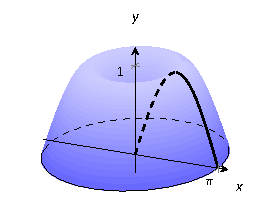
\includegraphics{figures/figshell4b}
\caption{Graphing a region in Example~\ref{eg:6.2.4}.} \label{F:6.2.Ex4b}
\end{marginfigure}